% !TEX root = main.tex
\code{My Python Snippet}{Python}{snippets/test.py}
\code{My C Snippet}{C}{snippets/test.c}

\begin{figure}
    \begin{center}
    % Generated with LaTeXDraw 2.0.8
% Sun Mar 31 15:28:25 CEST 2013
% test coment
% \usepackage[usenames,dvipsnames]{pstricks}
% \usepackage{epsfig}
% \usepackage{pst-grad} % For gradients
% \usepackage{pst-plot} % For axes
\begin{figure}
\scalebox{1} % Change this value to rescale the drawing.
{
\begin{pspicture}(0,-1.4475)(6.685,1.5525)
\pscustom[linewidth=0.04]
{
\newpath
\moveto(5.74,1.0375)
\lineto(6.28,0.7475)
\curveto(6.55,0.6025)(6.665,0.1875)(6.51,-0.0825)
\curveto(6.355,-0.3525)(5.9,-0.5375)(5.6,-0.4525)
\curveto(5.3,-0.3675)(4.82,-0.1375)(4.64,0.0075)
\curveto(4.46,0.1525)(4.405,0.4625)(4.53,0.6275)
\curveto(4.655,0.7925)(4.945,1.0175)(5.11,1.0775)
\curveto(5.275,1.1375)(5.515,1.1825)(5.59,1.1675)
\curveto(5.665,1.1525)(5.755,1.1125)(5.8,1.0375)
}
\pscustom[linewidth=0.04]
{
\newpath
\moveto(5.16,1.1575)
\lineto(4.97,1.4075)
\curveto(4.875,1.5325)(4.76,1.4625)(4.7,0.8775)
}
\pscustom[linewidth=0.04]
{
\newpath
\moveto(5.82,1.0575)
\lineto(6.04,1.2375)
\curveto(6.15,1.3275)(6.25,1.2825)(6.22,0.8775)
}
\pscustom[linewidth=0.04]
{
\newpath
\moveto(5.32,0.4175)
\lineto(5.44,0.3575)
\curveto(5.5,0.3275)(5.525,0.3075)(5.42,0.3375)
}
\pscustom[linewidth=0.04]
{
\newpath
\moveto(5.36,0.4175)
\lineto(5.53,0.3875)
\curveto(5.615,0.3725)(5.62,0.3975)(5.54,0.4375)
}
\pscustom[linewidth=0.04]
{
\newpath
\moveto(5.94,0.6175)
\lineto(6.13,0.6075)
\curveto(6.225,0.6025)(6.22,0.5625)(6.12,0.5275)
\curveto(6.02,0.4925)(5.915,0.4575)(5.9,0.4575)
}
\pscustom[linewidth=0.04]
{
\newpath
\moveto(4.46,0.6575)
\lineto(3.64,0.8975)
\curveto(3.23,1.0175)(2.56,0.7825)(2.3,0.4275)
\curveto(2.04,0.0725)(1.98,-0.3725)(2.18,-0.4625)
\curveto(2.38,-0.5525)(2.94,-0.6775)(3.3,-0.7125)
\curveto(3.66,-0.7475)(4.17,-0.6425)(4.32,-0.5025)
\curveto(4.47,-0.3625)(4.68,-0.1725)(4.74,-0.1225)
}
\pscustom[linewidth=0.04]
{
\newpath
\moveto(4.52,-0.4625)
\lineto(4.81,-0.6425)
}
\pscustom[linewidth=0.04]
{
\newpath
\moveto(4.28,-0.7025)
\lineto(4.76,-0.8625)
}
\pscustom[linewidth=0.04]
{
\newpath
\moveto(2.1,-0.0625)
\lineto(1.31,-0.2025)
\curveto(0.915,-0.2725)(0.305,-0.1575)(0.09,0.0275)
\curveto(-0.125,0.2125)(-0.17,0.3925)(0.0,0.3875)
\curveto(0.17,0.3825)(0.525,0.2875)(0.71,0.1975)
\curveto(0.895,0.1075)(1.265,0.0375)(1.45,0.0575)
\curveto(1.635,0.0775)(1.875,0.0875)(2.04,0.0575)
}
\usefont{T1}{ptm}{m}{n}
\rput(4.342656,-1.2925){Kocka domaci}
\end{pspicture} 
}
\label{label-kocka}
\caption{Caption - kocka}
\end{figure}


    \caption{Latex-Draw -> pstricks}
    \label{pic:pstricks} 
    \end{center}
\end{figure}

\begin{figure}
    \begin{center}
    % Graphic for TeX using PGF
% Title: /home/ondra/Diagram1.dia
% Creator: Dia v0.97.2
% CreationDate: Thu Aug  1 08:02:11 2013
% For: ondra
% \usepackage{tikz}
% The following commands are not supported in PSTricks at present
% We define them conditionally, so when they are implemented,
% this pgf file will use them.
\ifx\du\undefined
  \newlength{\du}
\fi
\setlength{\du}{15\unitlength}
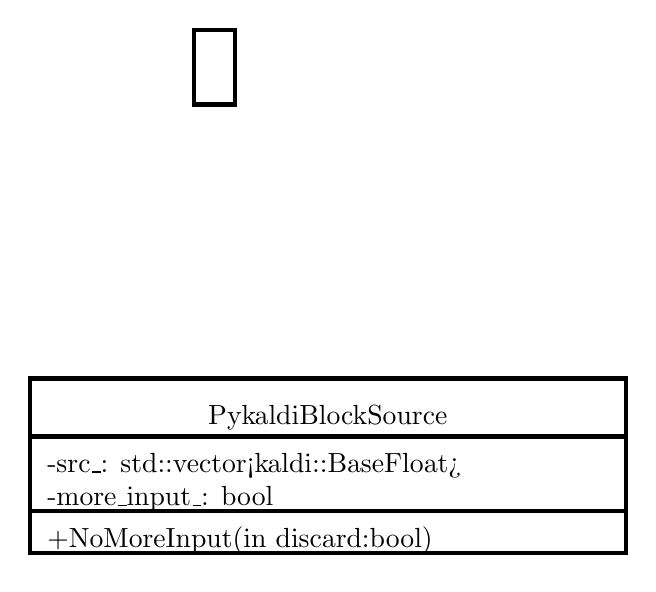
\begin{tikzpicture}
\pgftransformxscale{1.000000}
\pgftransformyscale{-1.000000}
\definecolor{dialinecolor}{rgb}{0.000000, 0.000000, 0.000000}
\pgfsetstrokecolor{dialinecolor}
\definecolor{dialinecolor}{rgb}{1.000000, 1.000000, 1.000000}
\pgfsetfillcolor{dialinecolor}
\pgfsetlinewidth{0.100000\du}
\pgfsetdash{}{0pt}
\definecolor{dialinecolor}{rgb}{1.000000, 1.000000, 1.000000}
\pgfsetfillcolor{dialinecolor}
\fill (13.250000\du,6.900000\du)--(13.250000\du,8.700000\du)--(14.250000\du,8.700000\du)--(14.250000\du,6.900000\du)--cycle;
\definecolor{dialinecolor}{rgb}{0.000000, 0.000000, 0.000000}
\pgfsetstrokecolor{dialinecolor}
\draw (13.250000\du,6.900000\du)--(13.250000\du,8.700000\du)--(14.250000\du,8.700000\du)--(14.250000\du,6.900000\du)--cycle;
% setfont left to latex
\definecolor{dialinecolor}{rgb}{0.000000, 0.000000, 0.000000}
\pgfsetstrokecolor{dialinecolor}
\node at (13.750000\du,7.995000\du){};
% setfont left to latex
\pgfsetlinewidth{0.050000\du}
\definecolor{dialinecolor}{rgb}{0.000000, 0.000000, 0.000000}
\pgfsetstrokecolor{dialinecolor}
\draw (13.750000\du,8.147500\du)--(13.750000\du,8.147500\du);
\pgfsetlinewidth{0.100000\du}
\pgfsetdash{}{0pt}
\definecolor{dialinecolor}{rgb}{1.000000, 1.000000, 1.000000}
\pgfsetfillcolor{dialinecolor}
\fill (9.300000\du,15.300000\du)--(9.300000\du,16.700000\du)--(23.660000\du,16.700000\du)--(23.660000\du,15.300000\du)--cycle;
\definecolor{dialinecolor}{rgb}{0.000000, 0.000000, 0.000000}
\pgfsetstrokecolor{dialinecolor}
\draw (9.300000\du,15.300000\du)--(9.300000\du,16.700000\du)--(23.660000\du,16.700000\du)--(23.660000\du,15.300000\du)--cycle;
% setfont left to latex
\definecolor{dialinecolor}{rgb}{0.000000, 0.000000, 0.000000}
\pgfsetstrokecolor{dialinecolor}
\node at (16.480000\du,16.250000\du){PykaldiBlockSource};
\definecolor{dialinecolor}{rgb}{1.000000, 1.000000, 1.000000}
\pgfsetfillcolor{dialinecolor}
\fill (9.300000\du,16.700000\du)--(9.300000\du,18.500000\du)--(23.660000\du,18.500000\du)--(23.660000\du,16.700000\du)--cycle;
\definecolor{dialinecolor}{rgb}{0.000000, 0.000000, 0.000000}
\pgfsetstrokecolor{dialinecolor}
\draw (9.300000\du,16.700000\du)--(9.300000\du,18.500000\du)--(23.660000\du,18.500000\du)--(23.660000\du,16.700000\du)--cycle;
% setfont left to latex
\definecolor{dialinecolor}{rgb}{0.000000, 0.000000, 0.000000}
\pgfsetstrokecolor{dialinecolor}
\node[anchor=west] at (9.450000\du,17.400000\du){-src\_: std::vector<kaldi::BaseFloat>};
% setfont left to latex
\definecolor{dialinecolor}{rgb}{0.000000, 0.000000, 0.000000}
\pgfsetstrokecolor{dialinecolor}
\node[anchor=west] at (9.450000\du,18.200000\du){-more\_input\_: bool};
\definecolor{dialinecolor}{rgb}{1.000000, 1.000000, 1.000000}
\pgfsetfillcolor{dialinecolor}
\fill (9.300000\du,18.500000\du)--(9.300000\du,19.500000\du)--(23.660000\du,19.500000\du)--(23.660000\du,18.500000\du)--cycle;
\definecolor{dialinecolor}{rgb}{0.000000, 0.000000, 0.000000}
\pgfsetstrokecolor{dialinecolor}
\draw (9.300000\du,18.500000\du)--(9.300000\du,19.500000\du)--(23.660000\du,19.500000\du)--(23.660000\du,18.500000\du)--cycle;
% setfont left to latex
\definecolor{dialinecolor}{rgb}{0.000000, 0.000000, 0.000000}
\pgfsetstrokecolor{dialinecolor}
\node[anchor=west] at (9.450000\du,19.200000\du){+NoMoreInput(in discard:bool)};
\end{tikzpicture}

    \caption{Dia -> tikz}
    \label{pic:tikz} 
    \end{center}
\end{figure}

\ac{BW}

% {{{
Lorem ipsum dolor sit amet, consetetur sadipscing elitr, sed diam nonumy eirmod
tempor invidunt ut labore et dolore magna aliquyam erat, sed diam voluptua. At
\ml{Did you know Lorem Ipsum before?}
vero eos et accusam et justo duo dolores et ea rebum. Stet clita kasd gubergren,
no sea takimata sanctus est Lorem ipsum dolor sit amet.
% }}}

What the \ac{ARPA} hack is it?
